\documentclass[12pt]{report}

%Links
\usepackage[hidelinks]{hyperref}
\usepackage{xcolor}

%Lang
\usepackage[italian]{babel}
\usepackage[utf8]{inputenc}{\tiny }

%Math
\usepackage{amsfonts}
\newcommand{\graffe}[1]{\left\lbrace #1 \right\rbrace}

%Toc
\setcounter{tocdepth}{2}

%Bib
\usepackage[numbers]{natbib}

%Graphics
\usepackage{graphicx}

\begin{document}
\section{Clustering}
La classificazione non-supervisionata, più spesso chiamata \textit{clustering}, consiste nel separare un insieme di dati non etichettati in insiemi, i \textit{cluster}, internamente omogenei.
\subsection{Ontologia}
\subsubsection{Obiettivi}
Gli obiettivi del clustering possono essere: la ricerca di conferma di ipotesi effettuate a priori, oppure esplorare lo spazio delle feature, per effettuare dei ragionamenti a posteriori. Può essere impiegato per effettuare delle statistiche differenziate su più gruppi, oppure per elaborare i dati differentemente a seconda del cluster a cui appartengono.
\subsubsection{Dati}
I dati in input sono detti \textit{pattern} e sono solitamente valori in uno spazio multidimensionale $\mathbb{R}^d$. Le caratteristiche dei dati significative per il clustering sono dette \textit{feature}: i \textit{pattern} possono essere presentati come array di \textit{feature} oppure le \textit{feature} possono essere proprietà calcolate a partire dai \textit{pattern}.
\subsubsection{Metrica}
Spesso, la diversità tra due pattern viene espressa come distanza all'interno dello spazio delle \textit{feature}: dovrà essere, quindi, definita la metrica di distanza da utilizzare (distanza euclidea, \textit{Manhattan}, \textit{Mahalanobis}, distanze di \textit{Minkowski}, \dots ).

\subsubsection{Algoritmo}
Per effettuare clustering esistono molti tipi di algoritmi, che si dividono principalmente in due classi: algoritmi gerarchici e algoritmi partizionali.

Gli algoritmi partizionali impongono una suddivisione dello spazio delle \textit{feature} in più sottoinsiemi, che sono i cluster: se ogni \textit{pattern} può appartenere ad un solo cluster si parla di \textit{hard clustering}, altrimenti, se ogni pattern può appartenere a più cluster con un grado di \textit{membership} si parla di \textit{soft clustering} o \textit{fuzzy clustering}.

Gli algoritmi gerarchici organizzano il dataset in una struttura ad albero dividendo cluster troppo disomogenei (algoritmi divisivi) o unendo cluster simili tra loro (algoritmi agglomerativi). I risultati del clustering gerarchico vengono rappresentati con un albero binario (o un dendrogramma) in cui il nodo radice è il dataset e le foglie sono gli oggetti: i nodi intermedi indicano le divisioni del dataset in cluster; il risultato finale del clustering si ottiene troncando il dendrogramma ad una certa altezza: si otterrà una foresta in cui ogni albero corrisponde a un cluster.

I vantaggi del clustering gerarchico sono l'indipendenza dall'inizializzazione e il fatto che non sia necessario specificare a priori il numero di cluster. Però, sono poco robusti (molto sensibili a rumore e agli outlier), non riconsiderano le scelte già fatte (l'errata classificazione di un punto non viene mai corretta), hanno costo computazionale almeno quadratico ($O(N^2)$) e tendono a creare cluster sferici e fenomeni di inversione.

\subsubsection{Validazione}
Qualsiasi sia la strategia utilizzata, devono essere applicate delle procedure consolidate di validazione del clustering, per confermare la fondatezza del risultato ottenuto.

\subsection{Quad-Tree Decomposition}
\begin{figure} \centering
	\caption{Esempio di utilizzo di \textit{quad-tree decomposition} per la compressione di un'immagine raster binaria}
	\label{fig:qtdecomp}
	\ \newline 
	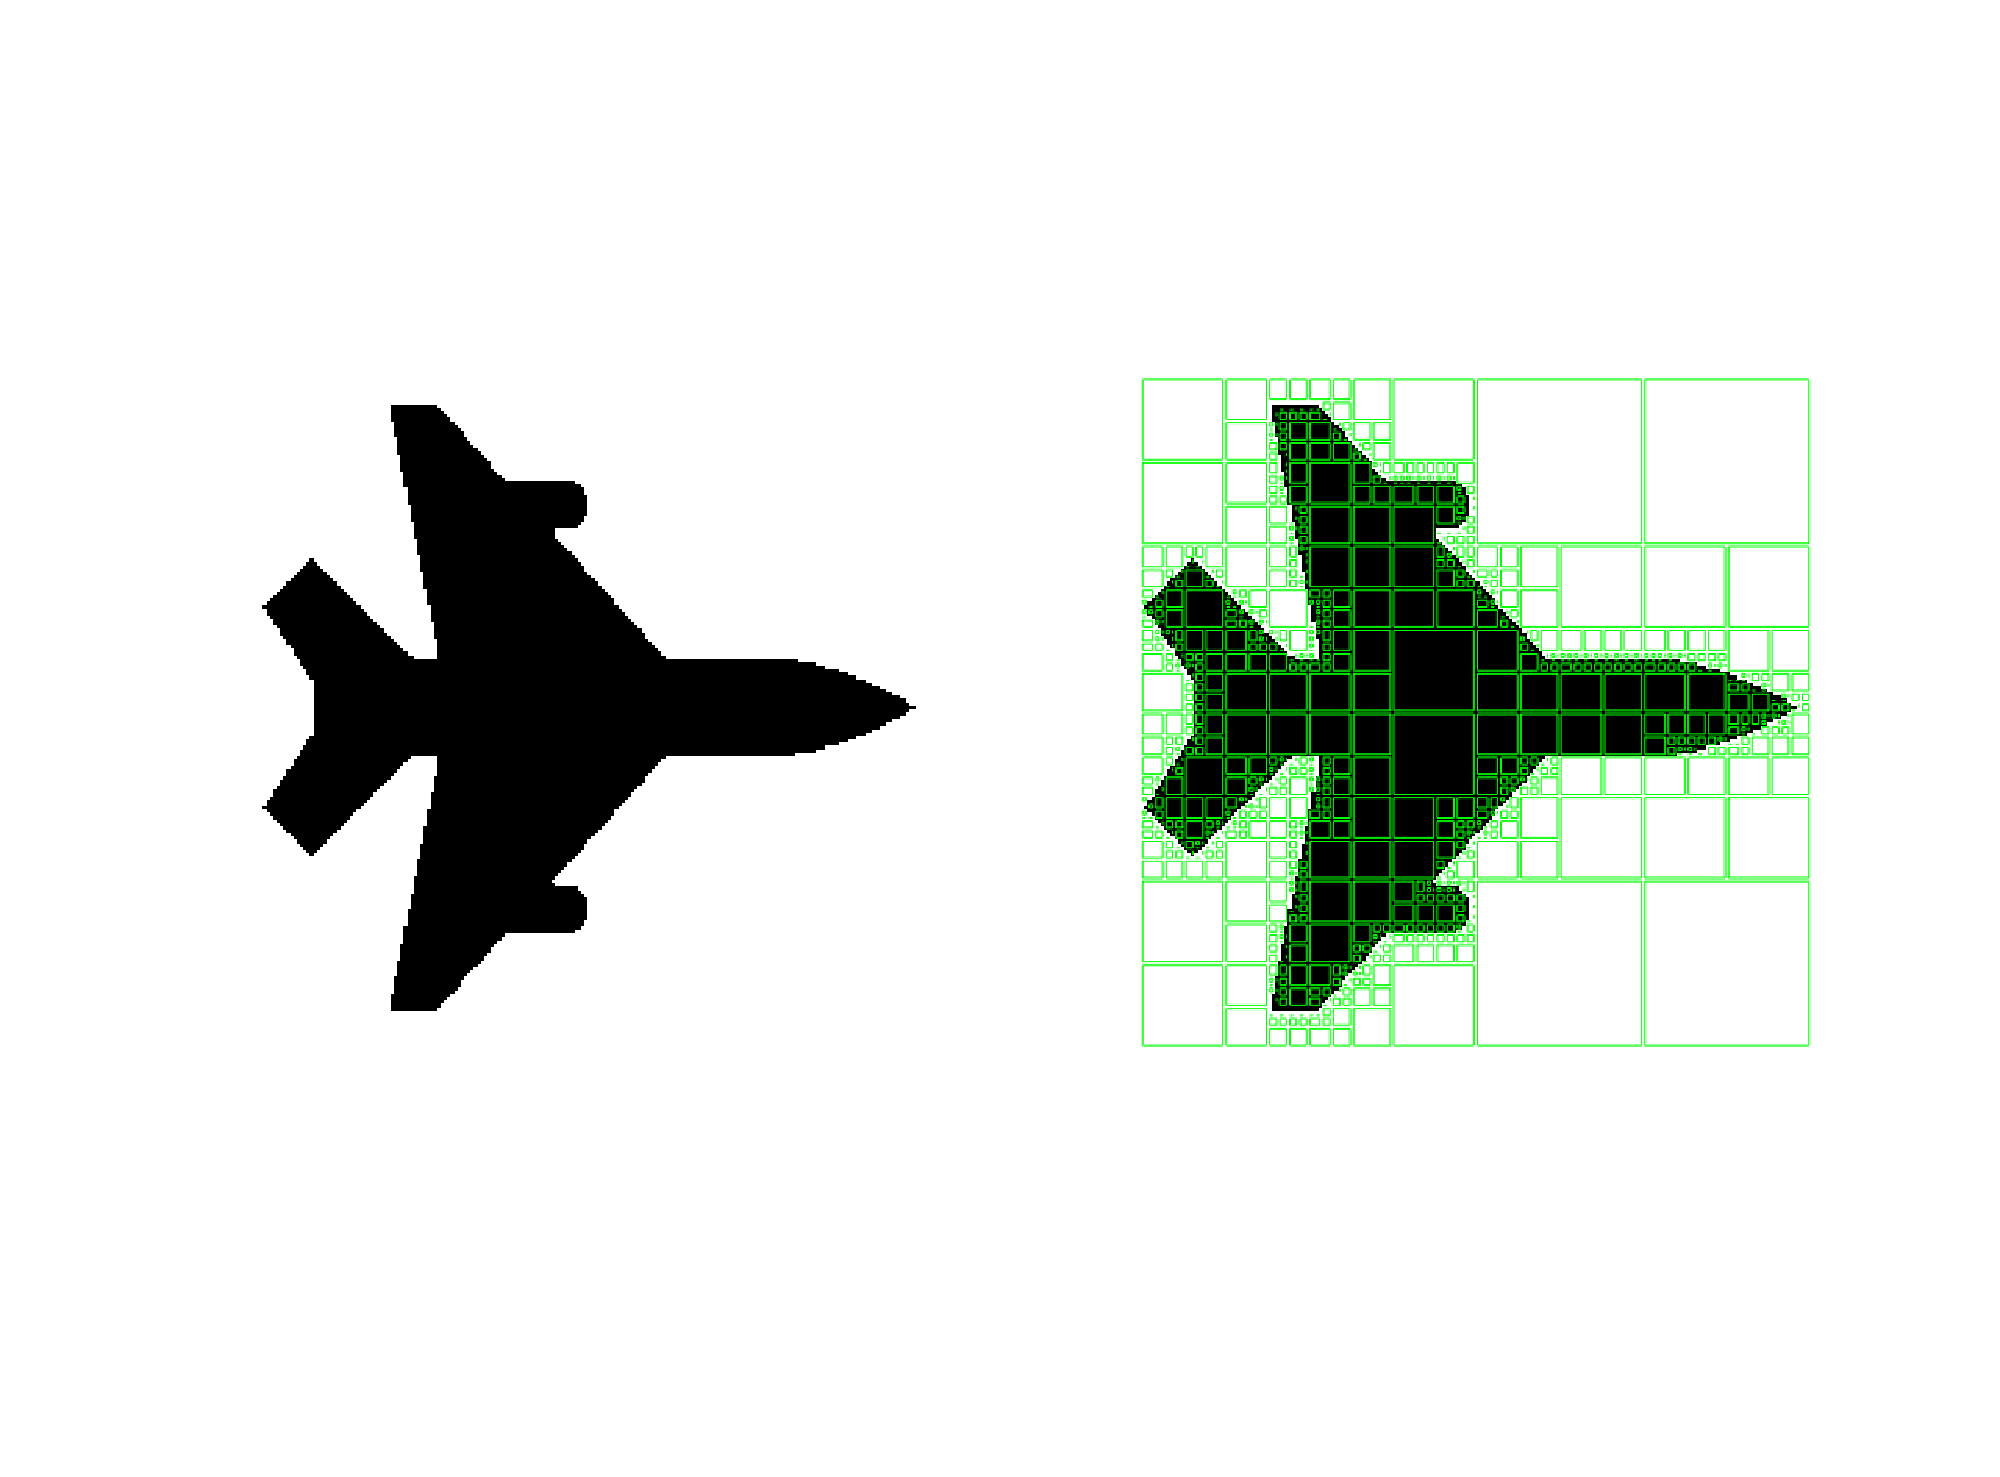
\includegraphics[width=\textwidth,trim={1.25in 2.5in 1.25in 2.5in},clip]{../images/qtdecomp.pdf}
\end{figure}
Con il termine \textit{quadtree} si indica una classe di strutture dati basate sulla decomposizione ricorsiva dello spazio: essi possono variare per il tipo di dati rappresentati, per il criterio che guida la decomposizione e la risoluzione (che può essere variabile o fissa). È un algoritmo gerarchico divisivo.

Il più comune approccio di tipo \textit{quad-tree decomposition} si basa sulla successiva divisione di un immagine in quattro quadranti di uguali dimensioni (come nell'esempio in figura~\ref{fig:qtdecomp}): un quadrante viene suddiviso solo se i pixel al suo interno sono disomogenei. Il nodo radice è l'intera immagine e il caso degenere della ricorsione è costituito dal singolo pixel (indivisibile). Occorre definire cosa si intende per disomogenei: per immagini binarie si può dire che ogni quadrante è omogeneo solo se tutti i pixel hanno lo stesso valore, per immagini RGB si può imporre una soglia di varianza.

\end{document}